\documentclass[xcolor={dvipsnames}]{beamer}

\mode<presentation> {
    \usepackage[utf8]{inputenc}
    \usepackage[T1]{fontenc}
    \usepackage[brazil]{babel}
    \usepackage{csquotes}

    \bibliographystyle{plain}

    \usetheme{Madrid}
    \usecolortheme{ipbutfpr}

    \setbeamertemplate{caption}[numbered]
    \setbeamertemplate{bibliography item}{\insertbiblabel}
    \setbeamertemplate{frametitle continuation}{\gdef\beamer@frametitle{}}

    \setbeamertemplate{footline}{
        \leavevmode%
        \hbox{%
            \begin{beamercolorbox}[wd=.4\paperwidth,ht=2.25ex,dp=1ex,center]{author in head/foot}%
                \usebeamerfont{author in head/foot}\insertshortauthor
            \end{beamercolorbox}%
            \begin{beamercolorbox}[wd=.6\paperwidth,ht=2.25ex,dp=1ex,center]{title in head/foot}%
                \usebeamerfont{title in head/foot}\insertshorttitle\hspace*{6em}
                \insertframenumber{} / \inserttotalframenumber\hspace*{1ex}
            \end{beamercolorbox}
        }%
        \vskip0pt%
    }

    \setbeamertemplate{navigation symbols}{}
}

\usepackage[language=brazil, style=numeric, sorting=none]{biblatex}
\addbibresource{main.bib}
\makeatletter

\makeatother

\title[]{O modelo Encoder-Decoder aplicado em irregularidades verbais do Português Brasileiro}

\author[Beatriz Albiero]{Beatriz Albiero}

\institute[IPB]{\normalsize
    Prof. Dr. Marcelo Barra Ferreira (USP)\\
    \\

    \begin{figure}[htb]
        \centering
        
\includegraphics[width=0.49\textwidth]{images/logos/fflch-logo.png}
        
    \end{figure}
}

\date{\small
Mestrado em Letras \\ 29 de Novembro de 2019}

\begin{document}
    \frame{\titlepage}

    %----SLIDES----%
    \begin{frame}{Introdução}
	\framesubtitle{Contexto}
	\begin{itemize}
		\item Inspirada pelo controverso debate sobre a aquisição de verbos irregulares em inglês (\cite{chomsky:1968}, ~\cite{Pinker:1988},
~\cite{Albright2003RulesVA}, ~\cite{kirov:2018}), esta pesquisa tem como objetivo estudar o \textbf{processo de inflexão de verbos irregulares em português} sob a perspectiva do modelo computacional \textbf{Encoder-Decoder}.
		\pause
		\item <1->O debate: modelos de aquisição associativos \textit{vs} por regras.
		\pause
		\item <2->Como verbos irregulares podem ser agrupados de acordo com padrões fonéticos, é possível propor modelos associativos para aprender tais padrões. Alguns exemplos de tais grupos são:
	\end{itemize}
	
	\begin{enumerate}
    \item Bob\textbf{ear}: Bob\textbf{eio}, Bloqu\textbf{ear}: Bloqu\textbf{eio}, Chat\textbf{ear}: Chat\textbf{eio}
    
    \item  Agr\textbf{e}d\textbf{i}r: Agr\textbf{i}do, Cons\textbf{e}gu\textbf{i}r: Cons\textbf{i}go, Ins\textbf{e}r\textbf{i}:Ins\textbf{i}ro
    
    \item Cobrir: C\textbf{u}bro, Dormir: D\textbf{u}rmo, Engolir: Eng\textbf{u}lo
    \end{enumerate}


\end{frame}

\begin{frame}{Introdução: Objetivos}

Construir um modelo Encoder-Decoder para aprender o processo de inflexão de verbos irregulares do português.


\end{frame}

    \begin{frame}{Metodologia: Escopo}

\begin{itemize}
    \item<1->O escopo da pesquisa foi limitado ao estudo do \textbf{paradigma da primeira pessoa do singular no modo indicativo e no tempo presente}. Ex: (Eu) falo, gosto, ouço. \\
    \item<2->A tarefa proposta é a de prever uma forma verbal flexionada, dada uma forma primária (\textbf{Radical + Vocal Temática}). Por exemplo, para o verbo Amar:
    
    \begin{align*}
    \text{Am + a + r}\\
    \text{Radical + VT + Desinência de Infinitivo}\\\\ 
    \text{Am + a} \rightarrow \text{Amo} \\
    \text{Radical + VT} \rightarrow \text{Forma Flexionada}
\end{align*}
    
\end{itemize}

\end{frame}

\begin{frame}{Corpus}
\begin{itemize}
    \item<1->O \textit{corpus} produzido é composto por 423 verbos que foram marcados como pertencendo às famílias de verbos regulares (51\%) ou irregulares (49\%).
    \item<2->Dentro do escopo da família de verbos irregulares, foi possível identificar 15 subgrupos conforme a identificação de diferentes padrões de flexão.
\end{itemize}
\end{frame}

\begin{frame}{Modelo}

\begin{figure}
    \centering
    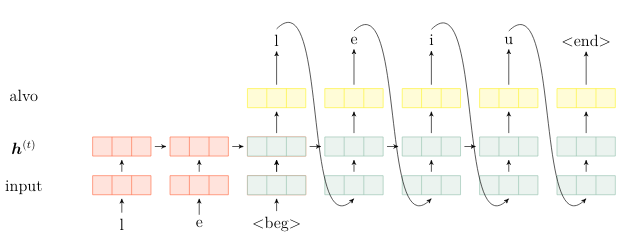
\includegraphics[width=0.8\textwidth]{images/metodologia/modelo.png}
    \caption{Esquema do Encoder-Decoder Desenvolvido}
    \label{fig:modelo}
\end{figure}

\end{frame}

\begin{frame}{Pré-Processamento}

\begin{figure}
    \centering
    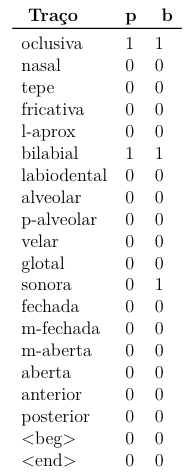
\includegraphics[width=0.2\textwidth]{images/metodologia/features.png}
    \caption{Exemplo de Codificação de fones}
    \label{fig:features}
\end{figure}
    
\end{frame}

\begin{frame}{Avaliação}

\begin{itemize}
    \item<1->A \textbf{Acurácia} foi a métrica escolhida para avaliar o modelo. Isso significa que o modelo deve prever corretamente todas as características fonéticas de cada fone do alvo.
    \item<2->Foram realizadas 30 análises K-fold com K=5.
\end{itemize}
    
\end{frame}
    \begin{frame}{Resultados}

\begin{figure}[H]
  \centering
  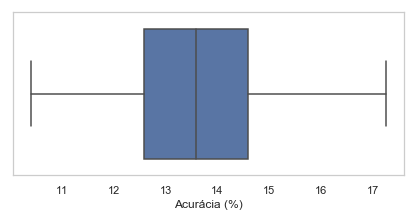
\includegraphics[width=0.6\linewidth]{images/results/mean_accuracy.png}
  \caption{Distribuição da Acurácia Para Todos os Verbos}
  \label{fig:acc}
\end{figure}

\end{frame}

\begin{frame}{Resultados}

\begin{figure}[H]
  \centering
  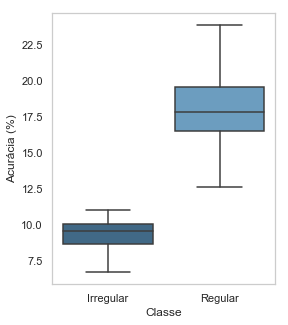
\includegraphics[width=0.4\linewidth]{images/results/boxplot_irregular_vs_regular.png}
  \caption{Distribuição da Acurácia por Classe Irregular e Regular}
  \label{fig:acc}
\end{figure}

\end{frame}

\begin{frame}{Resultados}

\begin{figure}[H]
  \centering
  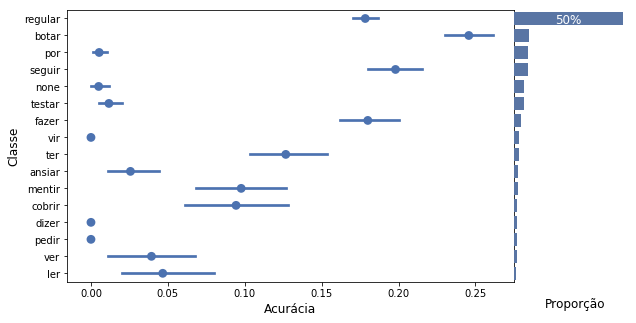
\includegraphics[width=0.9\linewidth]{images/results/proporxacc.png}
  \caption{Distribuição da Acurácia por Subclasse}
  \label{fig:acc}
\end{figure}

\end{frame}
    \begin{frame}{Conclusões}

\begin{itemize}
    \item<1->A acurácia máxima atingida pelo modelo foi de 17\% considerando todos os verbos do corpus ($73/423$). 
    \item<2->O tamanho do corpus é provavelmente incompatível com a arquitetura do modelo.
    \item<3->Ocorreram 32 erros de super-regularização.
    \item<4->A acurácia pode não ser uma boa métrica para este experimento, pois não captura o número de traços fonéticos previstos corretamente.
\end{itemize}


\end{frame}

\begin{frame}{Sugestões para Trabalhos Futuros}

\begin{itemize}
    \item<1-> Aumentar o corpus. 
    \item<2-> Tentar modelos de atenção (Transformers).
    \item<3-> Realizar testes psicolinguísticos.
\end{itemize}

\end{frame}

\begin{frame}{Aprendizados}

\begin{itemize}
    \item<1->Python
    \item<2->Fonética e Teorias de Aquisição
    \item<3->Aprendizado de Máquina e Ciência de Dados
    \item<4->Pesquisa

\end{itemize}

\end{frame}

\begin{frame}{Contribuições}

\begin{itemize}
    \item<1->Corpus 
    \item<2->Resultados dos Experimentos
    \item<3->Divulgação Científica:
    \begin{itemize}
        \item<4->IV Workshop do GLIC 2017 (oral)
        \item<5->ENAPOL XXI \& XXII (2018 e 2019)(oral)
        \item<6->PROPOR 2018 (pôster)
        \item<7->Khipu AI 2019 (pôster)
    \end{itemize}
\end{itemize}

\end{frame}

    %--------------%

    \frame{\titlepage}

    \section{Referências}
    \begin{frame}[allowframebreaks]
    \frametitle{Referências}
        \printbibliography
    \end{frame}

\end{document}
